% Guidance - 3 pages
% A technical description of the problem in terms of the requirements given,
% expanded into a discussion and highlighting likely implied technical aspects
% and challenges that need/needed to be tackled
\section{Description of Problem and Requirements}
The Embedded Systems Project consisted of two main sections: a group solution 
to a predetermined problem, and an individual extension to the group's work, 
left up to each person to determine. Both sections of the project involved 
embedded systems software development in the C programming language. 

The target platform of the development is an ARM-based microcontroller, 
situated on a board of peripheral accessories. The microcontroller consists of 
an interface board coupled with the ARM cortex-M3 based LPC1768, providing easy 
interaction via USB cable to transfer binaries, and simplifying the process of 
serial communication [how-mbed-works].

- Description of Peripheral Accessories.
The mbed board is sat on a board of peripheral accessiories, as pictured below. 

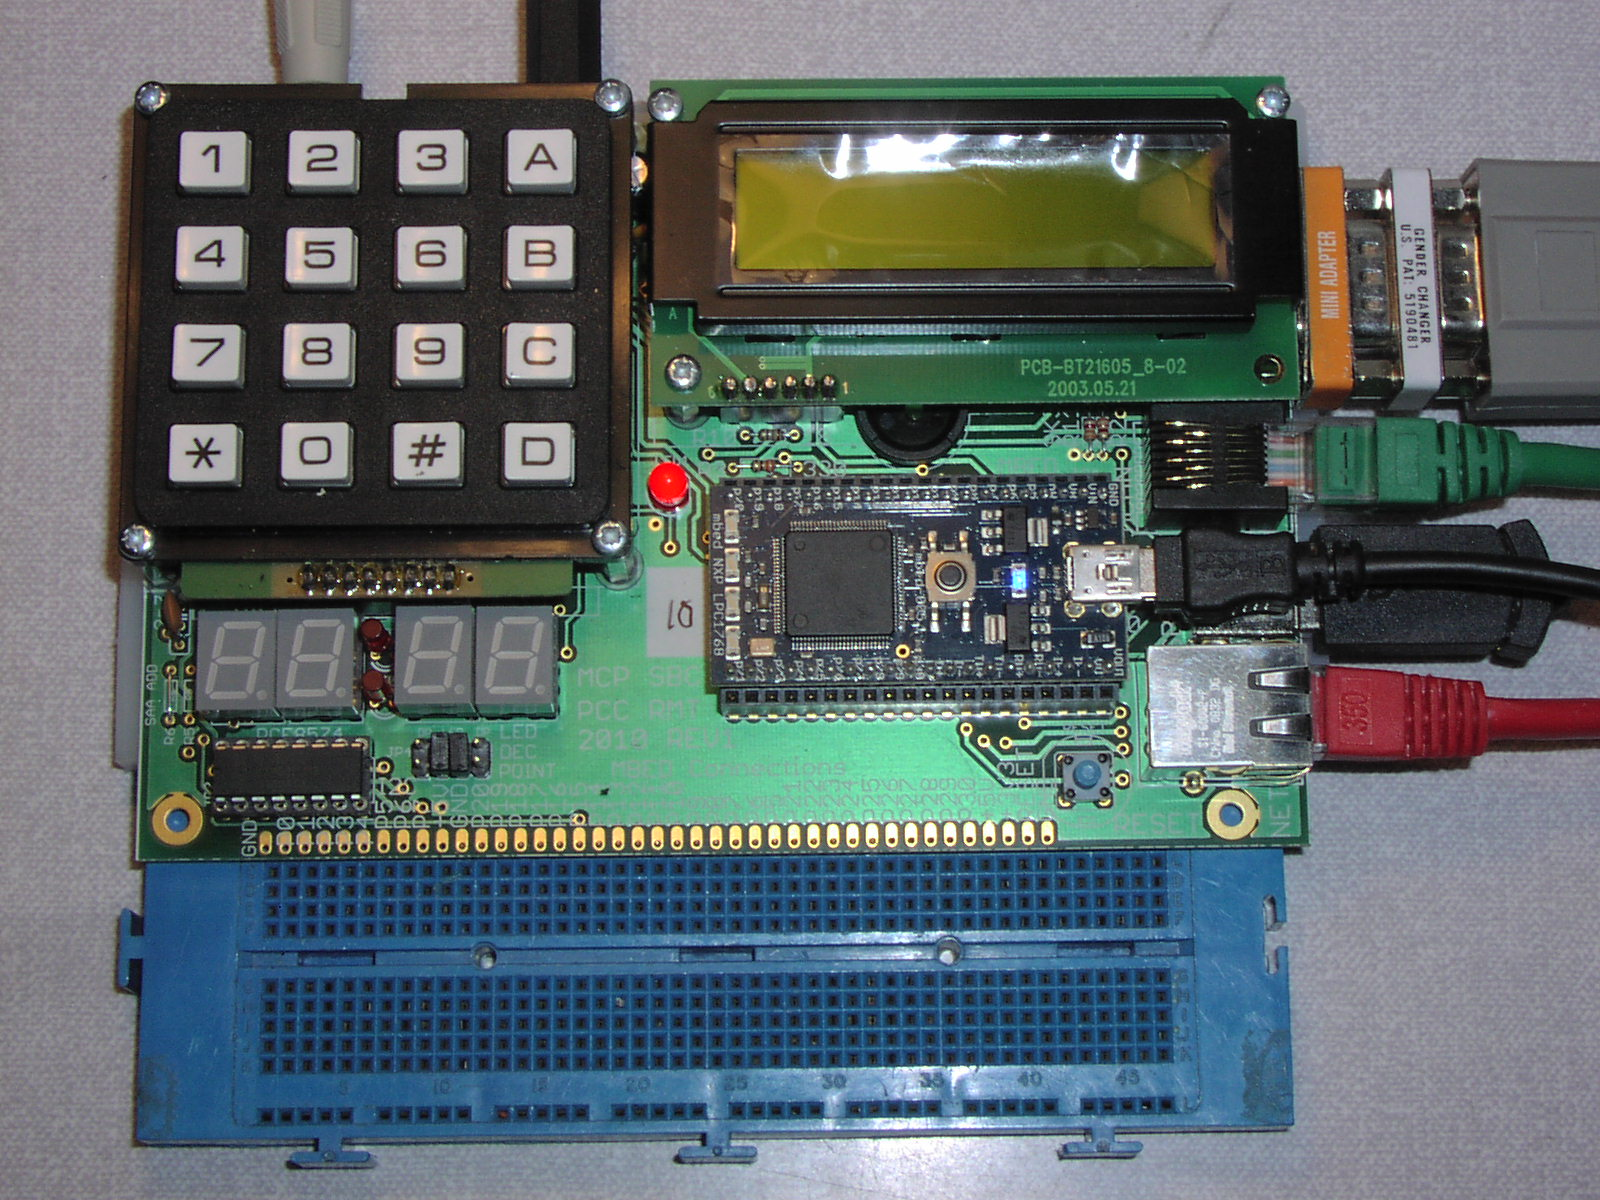
\includegraphics[width=0.80\textwidth]{./mbed_board}

- Description of Group Task.

- Requirements for the group task.


\section{Discussion of Technical Aspects and Challenges}

- Technical aspect 1 - CAN Bus 

- Technical aspect 2 - Syth code 

- Technical aspect 3 - User interfacing 

- Technical aspect 4 - ??

